\documentclass{article}
\usepackage[utf8]{inputenc}

\title{Mesterséges neuronhálók EA 1}
\author{Lőrincz András előadása alapján}
\date{2015 09 14}

\usepackage{natbib}
\usepackage{graphicx}

\begin{document}

\maketitle

\section{A tudományág kialakulása}
A mesterséges neuronhálók elméletének első lökését Donald O. Hebb, kanadai pszichológus adta 1949-ben, "The Organization of Behavior" című könyvében, melyben felvázolta a tanulásnak a neurális elméletét. Ebben azt posztulálta, hogy az agy biokémiai és elektromos folyamatokkal változtatja saját struktúráját. Amikor két neuron egy időben bocsát ki jelet, összeköttetésük erősödik, amikor koordinálatlanul tüzelnek, akkor gyengül (Hebb's postulate). \newline

\begin{figure}[h!]
\centering
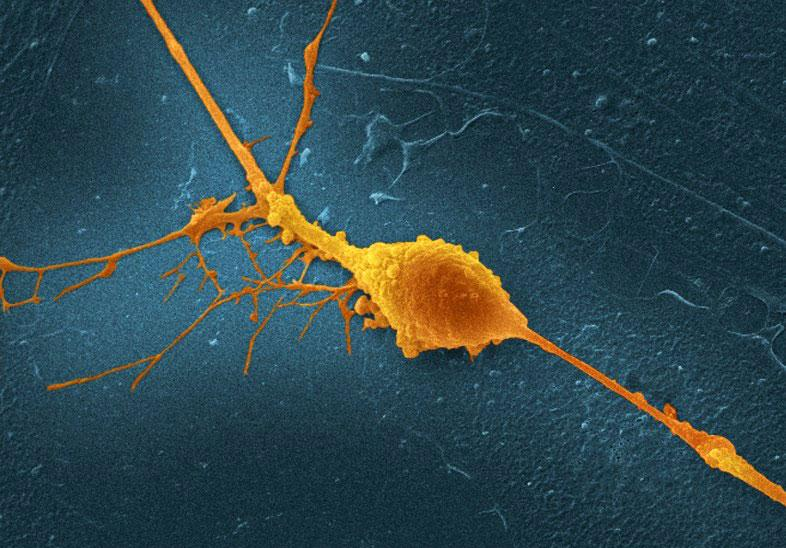
\includegraphics[width=\textwidth,height=\textheight,keepaspectratio]{realneuron.jpg}


\caption{A neuron elektronmikroszkópos képe}
\label{fig:realneuron}
\end{figure}

\begin{figure}[h!]
\centering
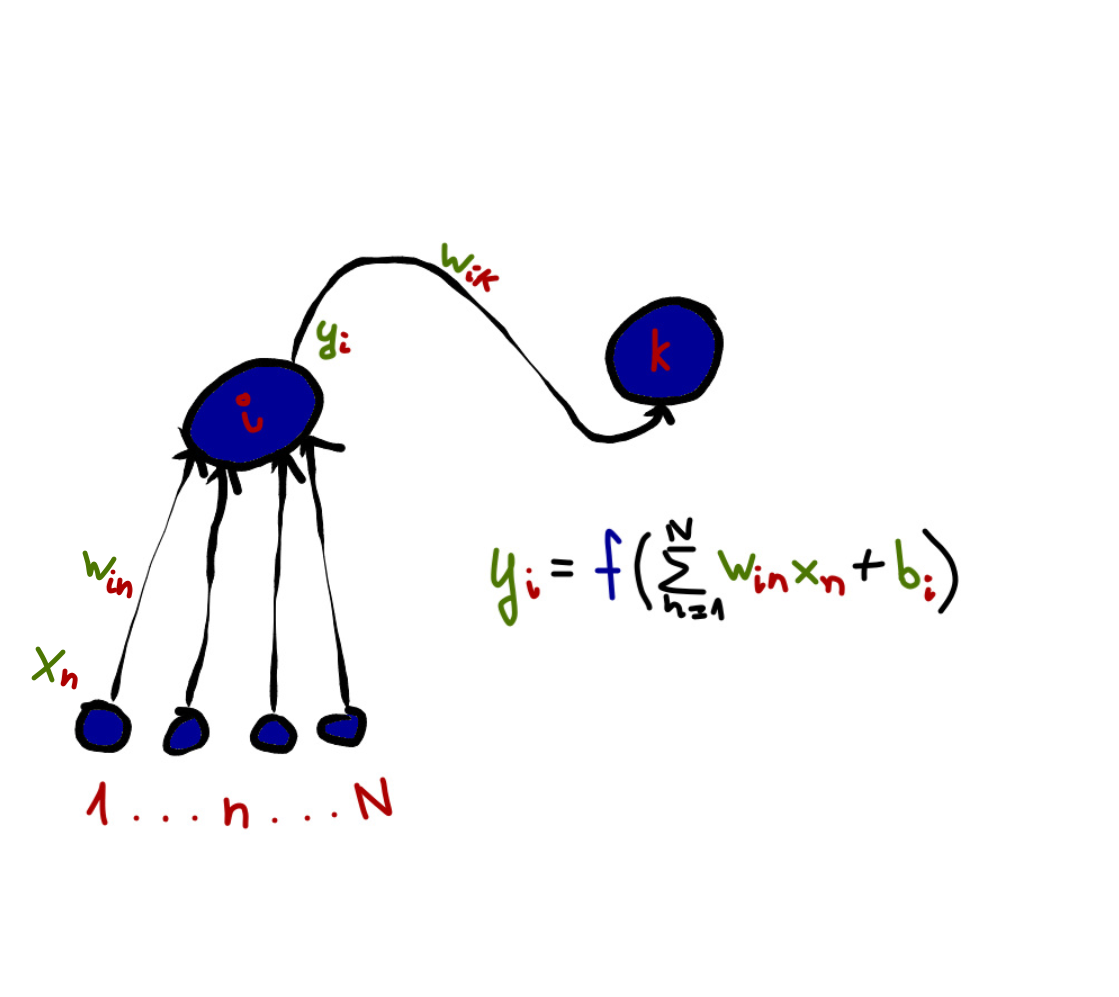
\includegraphics[width=\textwidth,height=\textheight,keepaspectratio]{abstractneuron.png}
\caption{A neuron absztrakciója}
\label{fig:abstractneuron}
\end{figure}

\section{Biológiai, pszichológiai alapok}
Az agy energiafelhasználása az egész test energiafelhasználásának közel 20\%-át teszi ki. Ennek felét a fehérállomány, felét a szürkeállomány adja. Agyunk nagyságrendileg $10^{11}$ neuront tartalmaz, de közel sem használja ki az összes kapcsolódási lehetőséget, csak $10^{14}$ kapcsolattal rendelkezik, ami neurononként 1000 kapcsolatot jelent. \newline

\begin{figure}[h!]
\centering
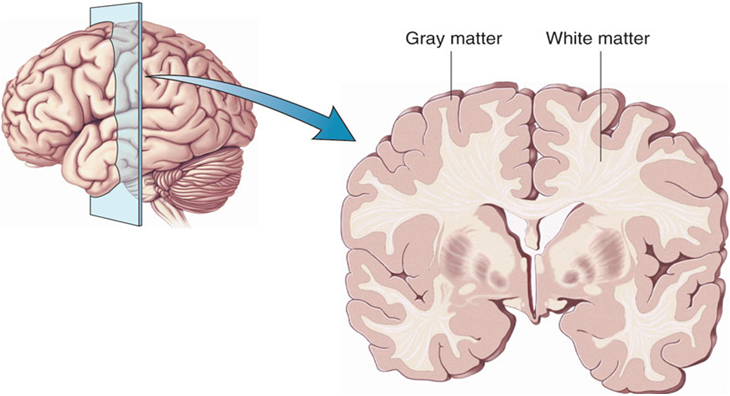
\includegraphics[width=\textwidth,height=\textheight,keepaspectratio]{brain.png}
\caption{Az agy fehér és szürkeállományának megoszlása}
\label{fig:brain}
\end{figure}

A neuronoknak a külvilágból érkező jeleket (input) meg kell kapniuk az érzékszerveiktől, és továbbítaniuk az izmoknak (output). Ez a folyamat akár fél másodpercet is igénybe vehet, és nagy a variancia köztük. Ezt a problémát az agy poliszinkronizációval oldja meg, azaz a jeleket prediktálja és szinkronizálja, ami után az eltérés már néhány ms-ra lecsökken. \newline

További problémát jelent, hogy az agynak interpretálnia kell a jelet valahogyan, értelmes végeredményt kell kapnia. Ez paradoxonokhoz vezet. Pl. vegyünk két különböző képet (majom és banán), és vetítsük a jobb és bal retinára őket egyszerre. Ekkor azt fogjuk tapasztalni, hogy a tesztalanyunk ahelyett, hogy egy összemosódott képet látna a kettő keverékéből, kb. 700ms késleltetéssel látja először az egyik, aztán a másik képet, folyamatosan váltakozva.\newline

A kísérlet lényegét bár nem olyan látványosan, de könnyen lehet szemléltetni az alábbi képpel (fig. 4). Mit látunk? Nyulat, vagy kacsát? \newline

\begin{figure}[h!]
\centering
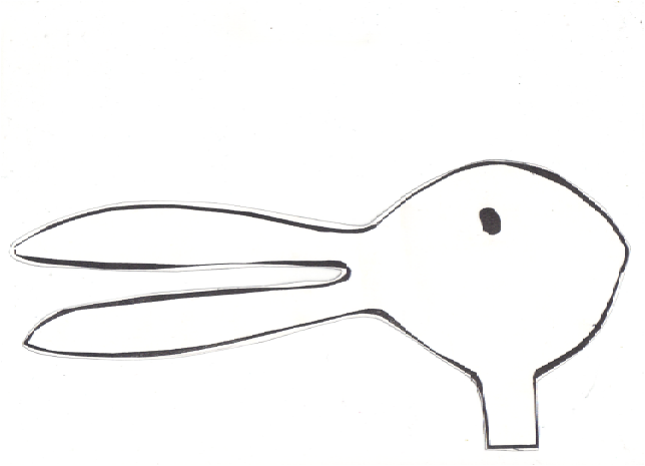
\includegraphics[width=\textwidth,height=\textheight,keepaspectratio]{duckrabbit.png}
\caption{An oldie but a goodie - It always comes back to the duck.}
\label{fig:duckrabbit}
\end{figure}

Ahhoz, hogy megértsük az inputokat milyen módon dolgozza fel az agy, egy hasznos segéd az úgynevezett "homunculus paradoxon", mely egy filozófiai eszköz elméletekben rejlő ellentmondások felismerésére. A paradoxon így szól: az agyunknak muszáj a környezetét és saját állapotát valahogyan reprezentálnia. A probléma az, hogy ezt a  reprezentációt aztán értelmezni is kell. Viszont magának az interpretációnak is valahogyan reprezentálva kell lennie. Ezt is interpretálni kell és így tovább. Ennek feloldása, hogy az értelmezést nem a reprezentáción végezzük, hanem maga a reprezentáció értelmezi azt amit reprezentál. Ha a reprezentációból le lehet vezetni az inputot, akkor értelmes, ha nem, akkor nem. \newline

\begin{figure}[h!]
\centering
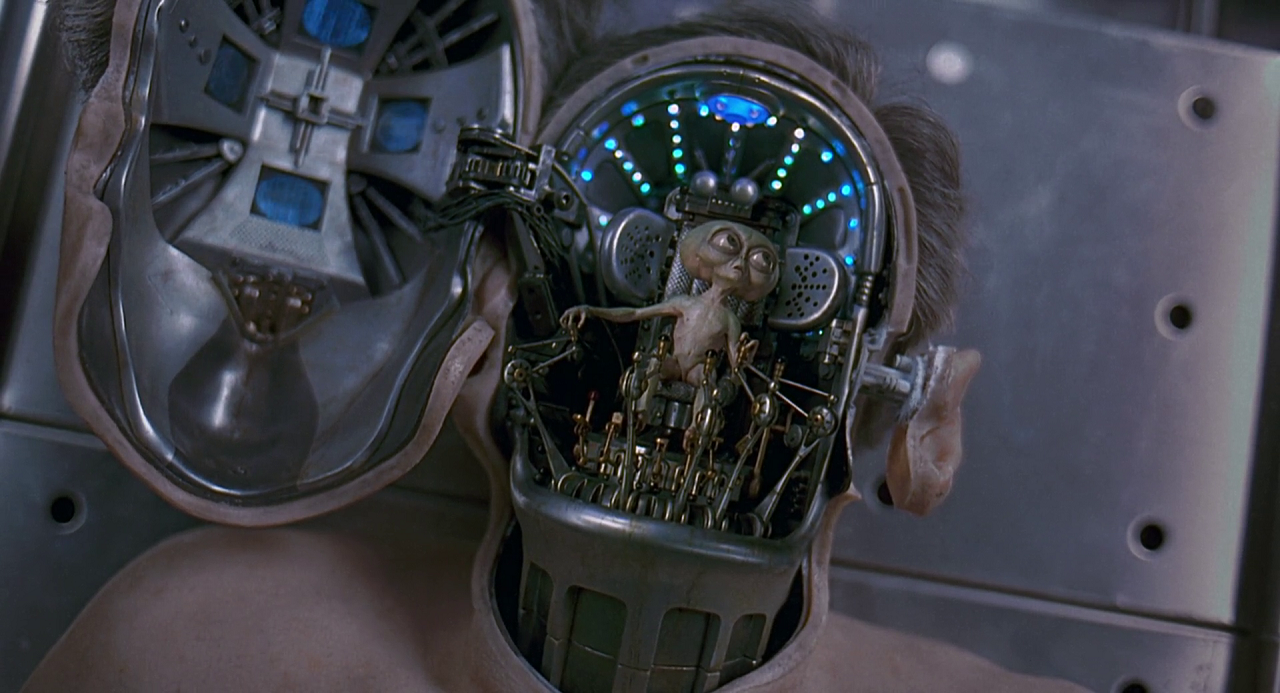
\includegraphics[width=\textwidth,height=\textheight,keepaspectratio]{homunculus.png}
\caption{Homunculus}
\label{fig:homunculus}
\end{figure}

\section{Feladatok osztályozása és kommunikálása}

TODO: Meg kell írni, ha már kikristályosodott a válasz.

\section{Humán vs. Gépi intelligencia}
A gépi intelligencia azoknál a feladatoknál tudja meghaladni a humán intelligenciát, ahol a feladat nehezen megoldható, és nehezen verifikálható.

\section{Fogalmak}
$y_i = f(\sum_{n=1}^N w_{in}*x_n + b_i)$ \newline

\textbf{Neuron:} $y_i$ az i. neuron képlete. Az inputokat megszorozza az i. súllyal, ezeket mind összeadja, eltolja a $b_i$-vel, végül az egész leképződik a kívánt range-be az aktivációs függvény (f) által. \newline

\textbf{Perceptron:} ???\\

\textbf{Súlyvektor:} az összes $w_ij$ súlyoknak a vektora. A kapcsolat erősségét jelzik.\\

\textbf{Küszöb:} képletünkben $b_i$ az i. küszöb. Ez segít eltolni függvényünket, hogy a neuron ne legyen túl érzékeny. \newline

A küszöböt fel lehet írni a súlyvektor komponenseként is. Ekkor képletünk leegyszerűsödik: $y_i = f(\sum_{n=0}^N w_{in}*x_n)$, ahol $x_0 = 1$, így megkapjuk az eredeti képletet $w_{i0} = b_i$ esetén. \newline

\textbf{Nemlinearitás:} A valódi neuronok nemlineáris dinamikus rendszerként működnek. Ennek a modellnek a reprezentálásához olyan függvényeket használunk, mint a sigmoid, vagy a tanh függvény. \newline

\textbf{Sigmoid:} $\frac{1}{(1+e^{-t})}$ \newline

\textbf{Tanh:} $\frac{e^x-e^{-x}}{e^x+e^{-x}}$ \newline

\textbf{Osztályozás:} A neurális háló outputja valami diszkrét osztályok egyikét adja vissza. Például angol ábécé karaktereinek felismerése: 26 elemű osztály valamelyikébe sorolja az inputot. \newline

\textbf{Short Term Memory (STM):} aktuális aktivitás-mintázat \newline

\textbf{Long Term Memory (LTM):} az összes információ a bementtől a kimenetig \newline
\newpage
\section{Ellenőrző kérdések}
\begin{enumerate}
\item{\textbf{Írd fel az origón átmenő hipersík egyenletét!}\newline
$y_i = f(\sum_{n=1}^N w_{in}*x_n)$}
\item{\textbf{Írd fel az origótól b távolságra levő hipersík egyenletét!}\newline
$y_i = f(\sum_{n=1}^N w_{in}*x_n + b_i)$}
\item{\textbf{Mi az a normálvektoros forma?}\\
???}
\item{\textbf{Mi az a perceptron?}\\
???}
\item{\textbf{Milyen komplexitású problémákat ismerünk, milyen módon különböztetjük meg azokat?}
\begin{enumerate}
\item nehéz megoldani, nehéz validálni 
\item nehéz megoldani, könnyű validálni
\item \textit{könnyű megoldani, nehéz validálni} Ezzel nem érdemes foglalkozni.
\item könnyű megoldani, könnyű validálni
\end{enumerate}

TODO: A kérdés második felére még hiányzik a válasz.
}
\item{\textbf{Milyen komplexítású problémákat/feladatokat érdemes kommunikálni?}\newline
A könnyen kommunikálhatóakat érdemes kommunikálni. :-) Azok közül is elsősorban a nehezen megoldható és könnyen kommunikálható problémákat.}
\end{enumerate}

\end{document}
